\documentclass[conference]{IEEEtran}
\usepackage{cite}
\usepackage{amsmath,amssymb,amsfonts}
\usepackage{algorithmic}
\usepackage{graphicx}
\usepackage{textcomp}
\usepackage{xcolor}
\def\BibTeX{{\rm B\kern-.05em{\sc i\kern-.025em b}\kern-.08em
    T\kern-.1667em\lower.7ex\hbox{E}\kern-.125emX}}
\begin{document}

\title{Emotion analysis in dataset}


\author{\IEEEauthorblockN{Meriem Aggoune}
\IEEEauthorblockA{\textit{dept. name of organization (of Aff.)} \\
\textit{name of organization (of Aff.)}\\
City, Country \\
email address or ORCID}
\and
\IEEEauthorblockN{ Lauri Heikka}
\IEEEauthorblockA{\textit{Faculty of Information Technology and Electrical Engineering} \\
\textit{Univ. of Oulu}\\
Oulu, Finland \\
lauri.heikka@student.oulu.fi}
\and
\IEEEauthorblockN{Anusha Ihalapathiranae}
\IEEEauthorblockA{\centerline{Faculty of Information Technology and Electrical Engineering} \\
\textit{Univ. of Oulu}\\
Oulu, Finland \\
anusha.ihalapathirana@student.oulu.fi}

}

\maketitle

\begin{abstract}
We document a series of experiments on using a variety of natural language processing methods to classify emotions conveyed by sentences. In particular, we compare word categorizations, semantic similarity approaches and machine learning approaches. The machine learning approaches consist of classification models based on bag-of-words representations and convolutional neural networks applied on word embeddings. Our results indicate that machine learning approaches outperform string matching and semantic similarity with a considerable margin. Within the machine learning approaches, convolutional neural networks with word embeddings provide an improvement in accuracy of around 3-5 percentage points over bag-of-words models. The best accuracy on a hold-out validation set, around 93\%, is achieved with a CNN approach using pre-trained word2vec embeddings. However, custom-trained word embeddings provide similar performance with less computational overhead.
\end{abstract}

\begin{IEEEkeywords}
natural language processing, text classification, sentiment analysis
\end{IEEEkeywords}

\section{Group info}
Group 10

Members: Meriem Aggoune, Lauri Heikka, Anusha Ihalapathiranae

Title: Emotion Analysis in Dataset

Github: https://github.com/MeriemLil/NLP\_Project

\section{Introduction}
Emotions are feelings that caused by a situation person interact with. It is also associate with person’s character, mood, personality and motivation. People express their feelings and emotions using verbally and non-verbally such as words, intonation of voice, facial expressions, gestures, and tears. Nowadays people tend to communicate their ideas, opinions, and feelings through social medias, Such as tweeter, facebook, instergram. People filled with lot emotions and they commonly use written text to express their emotions and feelings through social medias. Categorizing text into emotion types is known as emotion analysis. Sentiment analysis detect positive, negative, and neutral feelings from text and emotion analysis detect the types of feelings, emotion state, in the text \cite{emotiondetection}.

Emotion analysis takes major role in some applications which use emotion recognition, and it is a growing research area. There are supervised and unsupervised approaches can be found in this research area. A novel unsupervised context-based approach represents in \cite{unsupervisedemotiondetection} to detect emotions from text in sentence level. Their approached does not need any existing manually created lexicons and they used semantic relation between words and emotion type. They fine tune scores using syntactic dependencies within the sentence structure and proves this model provide more accurate results than other unsupervised approaches. Research carried out in \cite{jan2020emotion} paid their attention towards capturing semantic features in the text. Authors used distributional semantic model to calculate the semantic relatedness of the emotion in the text and they achieved accuracy of 71.79\% without training or annotation of data use.

A lot of research had been carried out on sentiment analysis and emotion analysis problem in many different languages. Bag-of-words representations, first suggested by Luhn in the 1950s \cite{luhn}, are an important advance, and still a commonly applied tool for natural language processing tasks like text classification. In these models, text is represented as a sparse feature matrix, where features represents the occurrences of a given word in a text. Earlier approaches involved counting the occurrences of words. Later, improvements have been suggested that offset the number of occurrences of a word in a given text by the frequency of the word's occurrence in other texts in the corpus \cite{tfidf}. The most notable of these approaches is the term frequency–inverse document frequency (tf-idf) weighting.

In a seminal paper on applying machine learning algorithms using a bag-of-words representation \cite{joachims-svm} propose the use of support vector regressions with the tf-idf matrix approach. Using this approach, they achieve notable improvements over the state-of-the-art benchmarks at the time. In a more recent example, \cite{chaffaretal}  demonstrate their work on supervised machine learning approach to recognize the emotion types using emotion annotated dataset which combined news headlines, fairy tales and blogs. They use bag of words and N-grams and proved that support vector machines classifier shows better performance and generalization than the other classifiers they used. 

\cite{kim-2014-convolutional} introduce convolutional neural networkds for text categorization. Similar concepts are explored by e.g. \cite{johnsonetal}, with a low complexity word level deep convolutional neural network for text categorization. \cite{dossantosetal} propose a new convolutional neural network that exploits from character to sentence level information to perform sentiment analysis of short texts. They found that combining small text with prior knowledge is effective.

Research in \cite{bert} introduce a new language representation model, BERT, a pretrained deep bidirectional representations from unlabeled text. They used conditioning on both information before and after a given word in all layers.BERT and successors inspired by it (see e.g. \cite{xlnet}), have massively improved the state-of-the-art in many language understandings tasks. For text classification, \cite{ bertclassification} used BERT provide general solution for BERT fine tuning in a text classification setting. Similarly, research on \cite{xu2020improving} improves the fine tuning of BERT using two effective mechanisms: self-ensemble and self-distillation.

In this work, we describe and empirically study a variety of approaches suggested in the text classification literature. Specifically, we focus on the task of identifying emotions from sentences, using a labeled dataset of 20 000 sentences spanning six different emotion states. The studied approaches include methods based on word categorization, semantic similarity and a wide range of different bag-of-words machine learning approaches. For these machine learning algorithms we also examine different methods of  preprocessing the sentences and forming bag-of-words representations. Finally we consider more recent advances in text classification by examining convolutional neural networks together with different approaches of forming word vector embeddings. 

In addition to the exhaustive amount of different approaches considered, we aim to provide as fair a comparison as possible across the different approaches. Importantly, we use a separate testing dataset for model selection and hyperparameter tuning, and then compare best performing approaches on a separate validation dataset. This avoids the problem of overfitting a test dataset, which is often bound to happen, when a large amount of candidate models and hyperparameter sets are considered.

\section{Data and Methodologies}
\subsection{Datasets and sources}
Our main dataset of interest is a labeled dataset of 20 000 sentences with between 3 and 66 words. The dataset is provided by \cite{kaggledata}. The sentences are labeled to convey one of six different emotions: fear, anger, joy, love, surprise and sadness. The dataset is collected following the approach of \cite{saravia-etal-2018-carer}. The sentences are tweets, and the emotion labels are hashtags at the end of the tweet. The sentences are preprocessed in that they contain no punctuation or special characters and all words are lowercase.

The dataset has a predefined split into training, test and validation samples, with 16 000, 2 000 and 2 000, respectively. Because the semantic similarity and string matching approaches do not employ any predictive modeling, in these sections we use the all 20 000 sentences to measure prediction accuracy. For the machine learning approaches, we use the training set for model training, the test set for model selection and hyperparameter tuning, and reserve the validation dataset as a final benchmark, to ensure a fair comparison accross approaches.

In addition, we use pre-trained, 300-dimensional word2vec embeddings  from \cite{mikolov2013distributed} and pre-trained fastText embeddings from \cite{bojanowski2016enriching}. Both datasets consist of 300-dimensional word embeddings, with embeddings for 3 and 1 million english words, respectively. For the string matching, we use the Harvard General Inquirer dataset, which contains categorizations for around 11 000 english words.

\subsection{Harvard Inquirer and String Matching}
The first method we explore is to categorize each word in Harvard General Inquirer \cite{harvardgeneralinquirer} to each emotion type. We use a filtering technique to this categorization. To identify words related to love emotion, we include Harvard General Inquirer words with that are labeled Affil label and exclude words associated with Negative label. The categories used for all six labels is reported in Table~\ref{taba3}. We store this information into a database and then compute the occurrences of words associated with each label for each sentence and predict the label of a sentence to be the category with the highest number of words.

\subsection{Empath Client Categories}
The next method we explore is to use the Empath Client \cite{empathclient}, a text analyzing tool with a pre-buildt category set. We identify categories related to each sentence using the Empath client. Then for all the identified categories, we compute empath category similarity with each label using the concept of lowest common hypernymy. We then associate each category provided by the Empath client with the emotion that has the highest similarity. Then, we use the label assigned to each category of a sentence to identify the label that has the highest number of occurrences. The emotion is predicted to be this label. The empath client categorization has a category for each of our labels as well, so we also experiment using only the exact emotion category.
\subsection{Semantic Similarity}
We pre-processed our dataset by tokenizing, removing stop words and adding position tags. Then we evaluate the semantic similarity between each emotion category and every sentence in the pre-processed dataset as the arithmetic average of Wu and Palmer similarity. We calculate it using two scenarios, taking only the first synset of the emotion category and taking mean of all synsets of the emotion categories.
\subsection{SentiStrength Sentiment Scores}
As part of the project specification, we also use the SentiStrength client \cite{sentistrength}, to compute sentiment scores. These can be potentially be used as an additional feature in any approach to distinguish between the negative and positive emotions. However, intuitively, the more difficult task is distinguishing between different positive emotions and between different negative emotions. For this purpose, the sentiment scores are unlikely to provide added benefit. Considering this, and the fact that the simple approaches perform quite poorly, we do not explore the effects of these sentiment scores onto the accuracy of different models. Sentiment scores are still delivered as part of the project database, as suggested in the project specification.

\subsection{Bag-of-Words Models}

Next, we conduct an empirical comparison on bag-of-words models. We treat this task as a model-selection and preprocessing strategy -selection exercise, and use the training dataset for training the machine learning algorithms and bag-of-words representations, and the test data for an out-of-sample comparison of models and preprocessing strategies. We then select the best performing preprocessing strategy and the best performing algorithm on the test dataset and further compare it to the CNN models described below, using the hold-out validation dataset. We also include a Logistic Regression and a Naive Bayes classifier as simple benchmark models.

The machine learning algorithms require some form of vectorization for the sentences. A bag-of-words model is a representation of documents (here sentences) that discards spatial information regarding the words in the document, and represents it as a collection of the number or frequency of occurrences for each word in a vocabulary. We consider the two most commonly employed bag-of-words representations: word counts\cite{luhn}, and term frequency-inverse document frequency\cite{tfidf}. It is important to note that we are, in a sense, misusing the term bag-of-words here, because the tf-idf is not a bag-of-words model. However, for the purpose of this research, we elect to use the term bag-of-words to describe any approach that disregards spatial information between words, to create a distinction between this branch of models and the convolutional neural networks that we introduce later.

Vectorization based on word counts is a simple approach, where the sentences are represented as a vector of length $length of vocabulary$, and the values correspond to the number of occurrences in the sentence. The tf-idf approach reweights the frequency of a word appearing in a document in proportion to it's frequency across the whole corpus. The tf-idf method has the advantage over word counts, that it adjusts for the over-emphasis on words that appear very often in the document corpus, and instead places emphasis on words that appear frequently in a given document, but not in other documents in the corpus.

The vocabulary used in vectorization is usually defined by the words occurring in the document corpus that is used for model training. Here, we use the vocabulary defined by the training dataset sentences. A common approach is to  restrict the vocabulary to some subset of the most frequent words occurring in the training corpus. We compare model performance between vocabularies restricted to 3000, 2000, 1000, 500 and 100 most frequent words, as well as using the full vocabulary. It is also possible to consider word n-grams to vectorize the sentences, but in order to keep the amount and complexity of model runs manageable, we elect to stick to single words.

Stop word removal is a common preprocessing strategy in forming bag-of-words models, where certain words are removed before vectorizations. Usually these are words that occur very commonly in the language studied (e.g. $the, what, who$. We consider two alternative sets of english stop words. The first is defined in the NLTK \cite{nltk} Python library and contains 127 commonly occurring english words. The second is the scikit-learn \cite{scikit-learn} default set of commonly occurring english words, and contains a larger set of 318 words. In addition we consider approaches with no stop word removal. Finally, we consider approaches with lemmatization versus no lemmatization. Lemmatization is the act of converting words in documents in to their dictionary form. For example, $dogs$ is lemmatized into $dog$ and $constructing$ is lemmatized to $construct$. This is intended to remove the sparsity in the bag-of-words vectors and improve the usefulness of features, by combining the inflected forms of a word. We use an NLTK \cite{nltk} pre-build implementation for stemming.

We consider six machine learning: logistic regression, naive bayes, support vector machines, decision trees, random forest and gradient boosting. In the interest of parsimony, we only provide a brief overview of the algorithms and direct the reader to alternative sources for more detailed descriptions.
\begin{itemize}
\item Naive Bayes classifiers model the probability of an input belonging to a class, conditioned on a given feature. The conditional probability is modeled separately for each feature and the conditional probabilities are combined to form a final estimate of the probability. The label with the highest posterior probability is assigned. In theory, Naive Bayes classifiers require an assumption of feature independece, but in practice the model can generalize well even when this assumption is not met.
\item Logistic regression, in its basic form uses a logistic function to linearly model a binary dependent variable, outputting a probability. Since we work in a multiclass setting, a one-vs-rest is applied, in which classifiers are trained for each of the six emotions. The predicted emotion label is then the class that has the highest probability. We also apply $l_2$ regularization, which penalizes large coefficients and prevents overfitting when many independent variables are considered.
\item Support vector machines can perform non-linear classification by transforming input of the data into higher dimensional space, where linear  an. For support vector classification, the multiclass setting is handled using a one-vs-one scheme, in which a binary classifier is trained for each pair of classifiers. When predicting a label, all classifiers make a predictions, and the label with the highest number of prediction is assigned as the predicted label. For the non-linear transformation, we use a radial-basis-function kernel. An $l_2$ regularization, penalty is applied in the support vector machine implementation as well.
\item Decision trees represent a flow-chart like structure that consists of nodes. Each node represents a decision rule that splits the decision space based on a feature value. Predictions are made by selecting a path down the decision tree based on feature values. Decision tree algorithms are trained top down by selecting a feature at each step that most effectively splits the training examples. We use the gini impurity criterion as a measure of the most effective split.
\item Random forest is an ensemble method, which combines multiple shallow decision trees and combines the predictions by individual classifiers into a voting scheme. Each decision tree is trained on the gini impurity criterion, using a random subset of features and training examples.
\item Gradient boosting is another ensemble method consisting of shallow decision trees. However, for gradient boosting decision trees are not trained independetly, but rather based on prediction errors made by the previously trained tree.
\end{itemize}

The full set of different approaches considered for the bag-of-words models is reported in table~\ref{tababw}. We consider, two vectorizers, six vocabulary sizes, three forms of stopword removal (including no stopwords), lemmatization and no lemmatization, and six machine learning algorithms, resulting in a total of $2 * 6 * 3 * 2 * 6 = 432$ model setups.

\begin{table*}[htbp]
\caption{Bag-of-Words models considered}
\begin{center}
\begin{tabular}{|c|c|}
\hline
\textbf{}&\multicolumn{1}{|c|}{\textbf{}} \\ 

\textbf{Parameter} & \textbf{\textit{Values}} \\ 
\hline
vectorizer & Count Vectorization, Tfidf Vectorization \\ 
\hline
stopwords & none, scikit-learn, nltk \\ 
\hline
Lemmatizing & yes, no \\ 
\hline
Max. features & Full, 3000, 2000, 1000, 500, 100 \\ 
\hline
Classifier & Naive Bayes, Logistic Regression, Support Vector Classification, Decision Trees, Random Forest, Gradient Boosting \\ 
\hline
\end{tabular}
\label{tababw}
\end{center}
\end{table*}

The classification methods discussed above all provide some hyperparameter options for model tuning. Even with parallel training, tuning the hyperparameters for different models becomes computationally costly, when such a large set of candidate models and preprocessing strategies are considered. Furthermore, we do not have a separate dataset for validation and hyperparameter tuning, as the validation dataset is reserved for the comparisons with convolutional neural network algorithms later. This can cause the comparison of algorithm performance on the test set to become a comparison of which algorithm is most capable of overfitting the test dataset, when a large set of hyperparameters are considered. For the reasons discussed above we do not perform any hyperparameter tuning in this model selection stage. Instead, for all machine learning algorithms, we use their default scikit-learn implementations with no changes to hyperparameters.\footnote{For full information on the default hyperparameters, we direct the reader to the scikit-learn documentation\cite{scikit-learn}. We use scikit-learn version 0.23.2.}. To form a meaningful comparison with the CNNs later, we tune the hyperparameters of the best performing algorithm on the test set before comparing with the validation dataset.

\subsection{Convolutional Neural Networks}

\subsubsection{Model architecture}

In the final stage replicate the convolutional neural network (CNN) architecture used in \cite{kim-2014-convolutional}. In this stage, the only preprocessing necessary for the sentences is tokenization and acquiring word vector embeddings for the tokenized sentences. The CNN architecture is outlined in fig.~\ref{fig1}. Sentences are represented as $n\times k$ matrices of word vector embeddings, where \emph{n} refers to the length of the sentences and $k$ to the dimension of the word vectors

\begin{figure*}[htbp]
\centerline{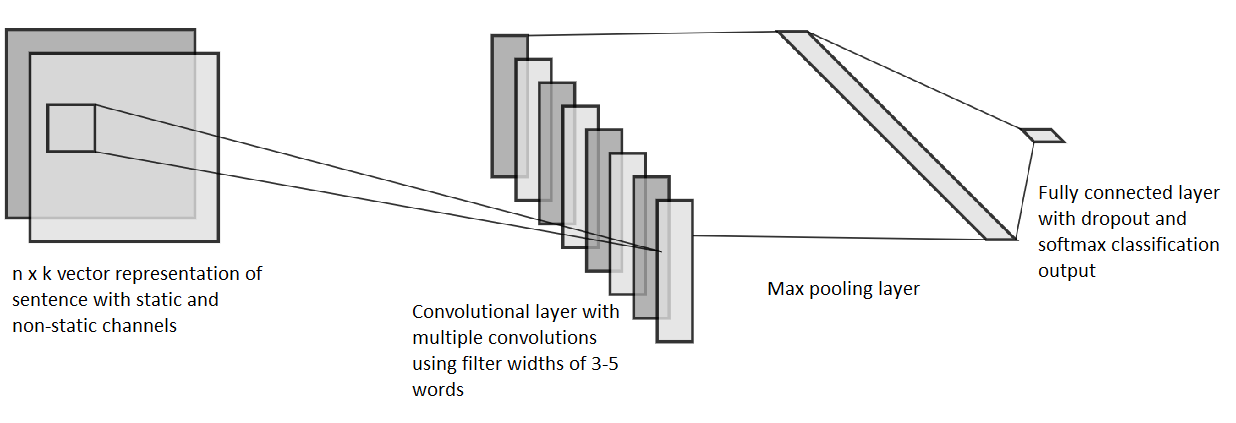
\includegraphics[width = \textwidth]{fig1.png}}
\caption{CNN model architecture}
\label{fig1}
\end{figure*}

All sentences are zero-padded to length $n$.
\footnote{A similar architecture is proposed in \cite{johnsonetal}, but one where sentences are not padded to a fixed length.  Note that, the application of max-pooling is likely to make the zero-padding inconsequential.}
Then a set of 1-dimensional convolutions are applied on the sentences. For each sentence, a feature $c_i$ is generated by the convolution
\begin{equation}
c_i = f(w * x_{i:i+h-1} + b)\label{eq1}
\end{equation}
where $h$ refers to the length of the convolution window, $w$ are the filter weights of the convolution operation, $b$ is an added bias term, and $f$ is a non-linear activation function. A feature map $c$ is then an $n-h+1$-dimensional vector of these features.

Equation \eqref{eq1} describes only one feature map produced by one convolution filter, while the model can consist of an arbitrary number of these feature maps. Then, for each feature map, max-pooling is applied, such that the largest feature value $c_{i-max}$ is selected. This operation produces a vector of final features with dimension equal to the number of feature maps used. These features are then connected to the final, 6-dimensional softmax output with a fully connected layer.

Like in \cite{kim-2014-convolutional}, we study three different variants of input to the CNN model. The first one involves keeping the inputted word embeddings as static. The second one is a model that sets the word embeddings as non-static, and the vectors are tuned for the task. The third variant of input is a multichannel, which inputs two sets of the same word embeddings and sets one set as trainable and keeps one set static. For selecting the best models, we treat this mode of input as a tunable hyperparameter and select the mode with best test set performance. However, we also report comparisons of accuracies between the different modes of input.

For regularization the original paper uses dropout on the penultimate layer. Dropout is a commonly used regularization method in neural networks. It hides each of the final features from the output layer with some probability $p$, preventing the co-adaptation of the different features. In addition, we experiment with another common method of avoiding overfitting; an $l_2$-norm regularization across the layer weights. The $l_2$ regularization penalizes large weight vectors, preventing overfitting.  Finally, following \cite{kim-2014-convolutional}, we also constrain the $l_2$ - norms of the weight vectors $w$ to be a maximum of a fixed size $s$. Note that the norm-constraint is most often applied to prevent an exploding gradients problem rather than to prevent overfitting.

\subsubsection{Word Embeddings}
The purpose of using word embeddings in the CNN model is to provide a $k$ dimensional numerical representation that can be input to the neural network. The general idea of these embedding model is to identify useful word embeddings by training a shallow neural network on a word prediction task using a large text corpus. Model training positions word vectors in the $k$-dimensional vector space such that similarities between word vector embeddings represent the semantic similarity between the words.

In \cite{kim-2014-convolutional}, pre-trained Word2Vec embeddings from \cite{mikolov2013distributed, mikolov2013efficient} are used. In addition to replicating this approach, we consider a few alternatives. First, we test pretrained fastText embeddings from \cite{bojanowski2016enriching, joulin2016bag}. Second, we explore explore training our own word2vec and fastText embeddings using the papers cited above.

 \cite{mikolov2013efficient} apply two approaches to training a word2vec model, a continuous bag-of-words (CBOW) model and a continuous skip-gram model. The idea for the CBOW model  is to train a shallow neural network to predict a current word in a sentence given a pre-specified window of words around it. The skip-gram model instead predicts the words around a given word wihin a pre-specified range in the sentence. The pre-trained word2vec vectors that we use in the experiments are trained using the skip-gram architecture. For our custom-trained embeddings, we instead use the CBOW model to provide a comparison.

FastText \cite{bojanowski2016enriching} is proposed as an extension to the word2vec model. The fastText model introduces subword information, in the form of character $n$-grams, by representing words as the sum of the vector representations of its $n$-grams. This means that or example if $n = 3$, then the word $what$ is represented by: $<wh, wha, hat, he>$ $n$-grams and the sequence $<what>$ itself. The authors in \cite{bojanowski2016enriching} argue that this allows to incorporate the internal structure of words and to produce more reliable representations for rare words.


\subsubsection{Hyperparameters and training}
 For the custom-trained word2vec and fastText models, we use a maximum distance between predicted words of five and early stopping on a generic word analogy evaluation task. Since this is a secondary objective, we do not explore alternative setups or model tuning for the word embedding task, and focus on tuning the CNN instead. We report results for pre-trained and custom-trained iterations of both word2vec and fastText models. As for the dimension of the word embeddings, we experiment with 50-, 100- and 300-dimensional word embeddings for the custom-trained word embeddings. With the pre-trained embeddings, we are restricted to the commonly available 300-dimensional word embeddings. 

For all CNN models, we use sentence length $n = 70$ and convolution windows $h$ of 3, 4 and 5.  following the original paper. We use a rectified linear unit (ReLU) activation function for the convolutions, and a softmax activation for the output layer. The original paper uses Adadelta \cite{adadelta} optimization, but we achieve faster convergence with an Adam \cite{adam} update rule. We train using mini-batches of 50 sentences, a learning rate of $10^{-3}$ and the cross-entropy loss function. We also employ early stopping based on the models cross-entropy loss on the test dataset.

For the input mode, we experiment with all three methods, static, non-static and multichannel inputs. As we have a number of other benchmarks, we omit the random initiation of the word embeddings.  The original paper uses a set of 100 convolutions. We treat the number of convolutions as a hypermeter, and experiment with from 50 to 250 convolutions. The original paper uses a dropout probability of 0.5. We tune the dropout parameter with values between 0.4 to 0.8. Note that the number of convolutions is applied for each of the three window lengths resulting in a total of $3 * number of feature maps$ convolutions. For the $l_2$ regularization parameter we try values between 0 and 0.001. The full set and ranges of the hyperparameters that we tune is reported in table~\ref{tabahp}. Note that the hyperparameter values represent the values attempted for any configuration. We do not attempt all possible configurations, but rather tune manually based on results from different model runs.

\section{Results and Discussion}

\subsection{Word categorizations and semantic similarity}

\begin{table}[htbp]
\caption{Word categorizations and semantic similarity accuracies}
\begin{center}
\begin{tabular}{|c|c|}
\hline
\textbf{Classifier}&\multicolumn{1}{|c|}{\textbf{Accuracy}} \\ 

\hline
Harvard String Matching & 0.336 \\ 
\hline
Empath Client & 0.160 \\ 
\hline
Empath Client with exact categories & 0.183 \\ 
\hline
Semantic Similarity - One synset & 0.269 \\ 
\hline
Semantic Similarity - All synset & 0.240 \\ 
\hline
\end{tabular}
\label{tab1}
\end{center}
\end{table}

\subsection{Model selection for bag-of-words}

Table~\ref{tab5} reports test set accuracies on the best performing iterations for each classifier and preprocessing strategy. For vectorization, we find only a miniscule improvement in accuracy of 0.002, when using tf-idf vectorization. As for the stop words, the best performing classifier uses the smaller nltk set of stop words. However, once again, the  performances are very similar across the stop word setups. Lemmatization does not seem to make much difference either, with no lemmatization achieving an accuracy improvement of 0.002 over lemmatization. The test set accuracy increases monotonically with the maximum size of the vocabulary. Performance is notably worse, when the vocabulary size is decreased below 1000 words, but beyond 2000 most frequent words, improvement in test set accuracy when increasing vocabulary size is miniscule.

\begin{table}[htbp]
\caption{Maximum accuracy on the test dataset across different bag-of-words setups}
\begin{center}
\begin{tabular}{|c|c|c|}
\hline
\textbf{}&\multicolumn{2}{|c|}{\textbf{}} \\ 
\cline{2-3}
\textbf{parameter} & \textbf{\textit{value}}& \textbf{\textit{score}} \\ 
\hline
vectorizer & CountVectorizer & 0.886 \\ 
\cline{2-3}
 & TfidfVectorizer & 0.888 \\ 
\hline
stopwords & nltk & 0.888 \\ 
\cline{2-3}
 & none & 0.878 \\ 
\cline{2-3}
 & sk & 0.884 \\ 
\hline
lemmatize & 0 & 0.888 \\ 
\cline{2-3}
 & 1 & 0.886 \\ 
\hline
max features  & 100 & 0.396 \\ 
\cline{2-3}
  & 500 & 0.728 \\ 
\cline{2-3}
 & 1000 & 0.865 \\ 
\cline{2-3}
  & 2000 & 0.880 \\ 
\cline{2-3}
  & 3000 & 0.886 \\ 
\cline{2-3}
 & All & 0.888 \\ 
\hline
classifier & DecisionTreeClassifier & 0.866 \\ 
\cline{2-3}
 & GradientBoostingClassifier & 0.849 \\ 
\cline{2-3}
 & LogisticRegression & 0.878 \\ 
\cline{2-3}
 & MultinomialNB & 0.859 \\ 
\cline{2-3}
 & RandomForestClassifier & 0.888 \\ 
\cline{2-3}
 & SVC & 0.876 \\ 
\hline
\end{tabular}
\label{tab5}
\end{center}
\end{table}

For the different machine learning algorithms test set performance is quite similar. The random forest algorithm outperforms others the next best classifier, logistic regression with $l_2$ penalty by 0.01. Even simple naivebayes achieves a test set accuracy just under 0.86 for the best iteration. Notably, gradient boosting, which we add beyond the project specification has the worst test set accuracy on the best iteration out of all classifiers. This is interesting, because gradient boosting has been shown to generally outperform other classification algorithms, though this does depend on data characteristics\cite{gbacc}.It also might be that the scikit-learn default hyperparameters are not well suited for our task. As our focus is an out-of-the-box model comparison, we do not do further experiment with alternative specifications for the gradient boosting.

\begin{figure}[htbp]
\centerline{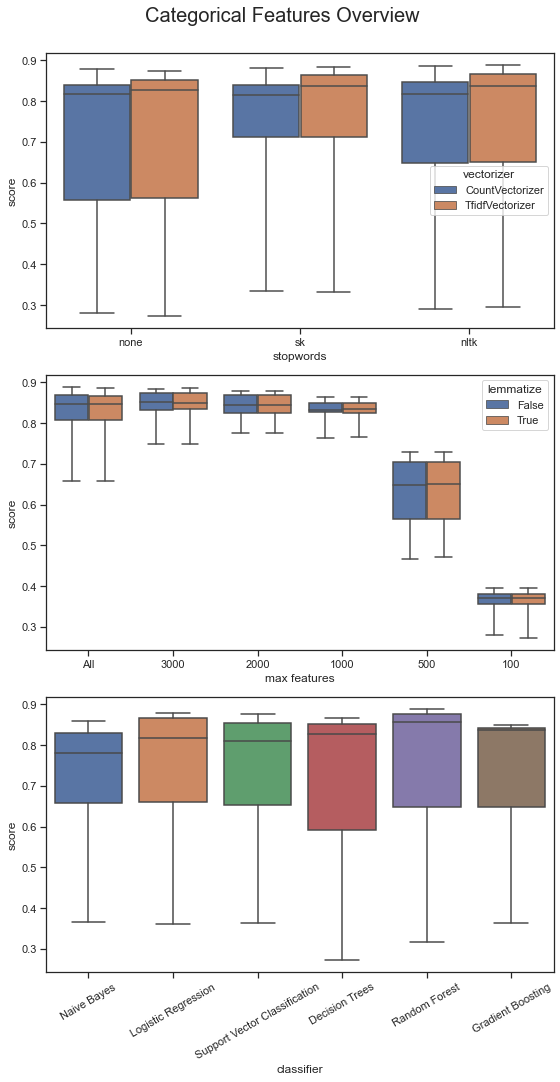
\includegraphics[width = 0.5 \textwidth]{fig2.png}}
\caption{Box plots of accuracies with different classifiers and preprocessing strategies.}
\label{fig2}
\end{figure}

To form a fair comparison preprocessing approaches and classifiers, it is important to take into account not just the best iteration, but all iterations that were experimented with. Figure~\ref{fig2}  shows boxplots describing the distribution of accuracies for each model and preprocessing setup. In addition, average accuracies are reported in the Appendix, table~\ref{taba5}. Tf-idf vectorization seems to have slightly higher test set accuracy across all quartiles and stop word specifications, although performance differences are small. For stop words, we see that the largest, scikit-learn set of stop words results in the most stable performance despite nltk stop words having the best performance. Again, lemmatization does not seem to have much effect on test set performance.

For the maximum size of the vocabulary, using the full vocabulary seems to result in less stable performance than using the most frequent 2000 or 3000 words. This is likely due to the fact that the large amount of feature results with the full vocabulary results in overfitting the training data. For example decision tree algorithms, are very prone to overfitting, when the tree depth is not restricted, which the case for deafult scikit-learn parameters. The lower quartiles and bounds shown in Fig.~\ref{fig2} for the decision trees support this intuition.The Random Forest remains the best performing algorithm, with over half of the iterations have an accuracy of around or above 0.85. Gradient boosting  likewise, has good berformance on the median, but it's accuracy seems restricted in the upper bound.

As mentioned, we treat this  bag-of-words model comparison as a model selection exercise, and select the best model to compare to the CNN models on the validation test set. For the preprocessing strategy, we select the scikit-learn stop words due to their more stable performance, despite nltk stop words having slightly higher maximum accuracy. Lemmatization seems to make no difference, so in the interest of parsimony, we do no lemmatization. We use tf-idf vectorization, with a maximum vocabulary size of 3000 words, since it seems to yield the best tradeoff between maximum accuracy and stability of the accuracy.

Random Forest is selected as the best algorithm. To make a fair comparison, we tune hyperparameter of the random forest on the test set. We tune the minimum samples per leaf node (1, 2, 3), minimum samples split by a node (values between 2 and 20) and the number of unique tree estimators (values between 100 and 2000). The parameters selected are, 1700 estimators, 4 minimum samples split, and 1 minimum sample per leaf node. In addition, we use Naive Bayes and Logistic Regression as simple benchmark models for the next step. We use the best selected preprocessing strategy, described above for all three benchmark algorithms.

\subsection{Validation set performance of best models}

Table~\ref{tab1} reports the accuracies on the test and validation datasets for the three benchmark models and CNN models with 4 different word embedding configurations. The CNN models all achieve validation accuracies between 0.925 and 0.93, while the best bag-of-words model, a tuned random forest achieves a 0.899 accuracy. The CNNs clearly outperform bag-of-words models in terms of accuracy. Hyperparameter tuning improves random forest performance on the test set very little, from the best accuracy of 0.888 in the previous section to 0.890. Validation set performance is slightly better, however at 0.899.

Which word embeddings are used, does not seem to matter much. Differences between the different models are very small\footnote{We do not establish statistical significance between the accuracy values. It is, however, likely that these differences are not statistically significant.}. The highest accuracy is achieved by pre-trained word2vec embeddings. However, embeddings trained from scratch on the training dataset achieve similar performance. Interestingly, the word embeddings trained from scratch achieve higher validation accuracy than pre-trained fastText embeddings. 

\begin{table}[htbp]
\caption{Validation and test set accuracies for best models}
\begin{center}
\begin{tabular}{|c|c|c|}
\hline
\textbf{}&\multicolumn{2}{|c|}{\textbf{Accuracy}} \\ 
\cline{2-3}
\textbf{Classifier} & \textbf{\textit{Validation}}& \textbf{\textit{Test}} \\ 
\hline
MultinomialNB & 0.681 & 0.694 \\ 
\hline
LogisticRegression & 0.872 & 0.864 \\ 
\hline
RandomForestClassifier & 0.899 & 0.890 \\ 
\hline
CNN fastText pretrained & 0.925 & 0.928 \\ 
\hline
CNN Word2Vec own & 0.928 & 0.929 \\ 
\hline
CNN fastText own & 0.928 & 0.931 \\ 
\hline
CNN Word2Vec pretrained & 0.930 & 0.928 \\ 
\hline
\end{tabular}
\label{tab1}
\end{center}
\end{table}

In table~\ref{tab1}, it is noteworthy that, the validation accuracy for naive bayes is only 0.681 for the preprocessing strategy selected in the model. This is much smaller than the best performing naive bayes models at the model selection stage. This is likely caused by the use of tf-idf vectorization. The naive bayes algorithm assumes  a multinomial discrete distribution, which count vectorization produces but tf-idf does not. However, a commonly accepted stylized fact is, that tf-idf matrices can also work well with naive bayes. In the interest of simplicity, we elect to use the best performing overall preprocessing strategy from the previous section for all algorithms. Furthermore, considering the test set performances reported in previous section, it is unlikely that naive bayes would have outperformed the CNNs or the tuned random forest. Accuracies on the test and validation datasets are very similar for all models. There seems to be no evidence in overfitting the test dataset. Note that the test dataset is not used for retraining the model, but only for hyperparameter tuning and model selection.

An important aspect to note, is that the word embeddings for all the best performing cnn iterations, reported in table~\ref{tab1} are re-trained in the model training, i.e. using the non-static and multichannel methods. A comparison of test set accuracies and test losses for the CNN models using different types of embeddings: multichannel, non-static and static, is reported in table~\ref{taba1}. The models with pre-trained word embeddings achieve best test set accuracy using to sets of embeddings, trainable and non-trainable, while the word embeddings trained from scratch benefit from using only one set of trainable embeddings. This is an intuitive result in the sense that, considering the small size of the dataset, the custom word embeddings are not likely to contain as semantically relevant information as the pretrained ones, which are trained using massive corpora.

Pre-trained vs. custom embeddings seem to affect the characteristics of an ideal model, even though they do not affect the performance very much. The selected hyperparameters for the CNN models are reported in table~\ref{taba4}. Noteworthy aspects are the fact that, the custom-trained embeddings benefit from a smaller word dimension of 50 compared to the 300, which is mandated by the pretrained vectors. Furthermore, stronger regularization with higher dropout and added $l_2$ regularization is applied on the custom embeddings. Table~\ref{tabfmaps} reports the best model and test set accuracy for different number of convolutions. The ideal number of convolutions seems to be 100 or 150 depending on the embeddings, after which performance slightly drops off.

Table~\ref{tab2} reports the class weighted precision and recall on the validation dataset for the three benchmark models and CNN models with 4 different word embedding configurations. Validation set confusion matrices for the best models for each emotion are reported in table~\ref{taba2}. The overall takeaway from the two tables is, that the model accuracies are not explained by class imbalances.

\begin{table}[htbp]
\caption{Validation precision and recall for best models}
\begin{center}
\begin{tabular}{|c|c|c|}
\hline
\textbf{}&\multicolumn{2}{|c|}{\textbf{Metric}} \\ 
\cline{2-3}
\textbf{Classifier} & \textbf{\textit{Precision}}& \textbf{\textit{Recall}} \\ 
\hline
MultinomialNB & 0.734 & 0.681 \\ 
\hline
LogisticRegression & 0.875 & 0.872 \\ 
\hline
RandomForestClassifier & 0.898 & 0.899 \\ 
\hline
CNN fastText pretrained & 0.926 & 0.925 \\ 
\hline
CNN Word2Vec own & 0.93 & 0.928 \\ 
\hline
CNN fastText own & 0.928 & 0.928 \\ 
\hline
CNN word2vec pretrained & 0.93 & 0.93 \\ 
\hline
\end{tabular}
\label{tab2}
\end{center}
\end{table}


\begin{table*}[htbp]
\caption{Confusion matrices}
\begin{center}
\begin{tabular}{|c|c|c|c|c|c|c|}
\hline
\textbf{}&\multicolumn{6}{|c|}{\textbf{Label}} \\ 
\cline{2-7}
\textbf{Classifier} & \textbf{\textit{joy}}& \textbf{\textit{sadness}}& \textbf{\textit{anger}}& \textbf{\textit{fear}}& \textbf{\textit{love}}& \textbf{\textit{surprise}} \\ 
\hline
CNN Word2Vec & 664$\;$$\;$$\;$$\;$  32 & 525$\;$$\;$$\;$$\;$26 & 254$\;$$\;$$\;$$\;$16 & 196$\;$$\;$$\;$$\;$34 & 158$\;$$\;$$\;$$\;$30 & 60$\;$$\;$$\;$$\;$5 \\ 

own & 40$\;$$\;$$\;$$\;$1264 & 25$\;$$\;$$\;$$\;$1424 & 21$\;$$\;$$\;$$\;$1709 & 16$\;$$\;$$\;$$\;$1754 & 20$\;$$\;$$\;$$\;$1792 & 21$\;$$\;$$\;$$\;$1914 \\ 
\hline
CNN fastText & 674$\;$$\;$$\;$$\;$38 & 531$\;$$\;$$\;$$\;$32 & 258$\;$$\;$$\;$$\;$25 & 171$\;$$\;$$\;$$\;$12 & 155$\;$$\;$$\;$$\;$22 & 67$\;$$\;$$\;$$\;$15 \\ 

own & 30$\;$$\;$$\;$$\;$1258 & 19$\;$$\;$$\;$$\;$1418 & 17$\;$$\;$$\;$$\;$1700 & 41$\;$$\;$$\;$$\;$1776 & 23$\;$$\;$$\;$$\;$1800 & 14$\;$$\;$$\;$$\;$1904 \\ 
\hline
CNN fastText & 664$\;$$\;$$\;$$\;$36 & 520$\;$$\;$$\;$$\;$17 & 259$\;$$\;$$\;$$\;$24 & 195$\;$$\;$$\;$$\;$35 & 148$\;$$\;$$\;$$\;$27 & 64$\;$$\;$$\;$$\;$11 \\ 

pretrained & 40$\;$$\;$$\;$$\;$1260 & 30$\;$$\;$$\;$$\;$1433 & 16$\;$$\;$$\;$$\;$1701 & 17$\;$$\;$$\;$$\;$1753 & 30$\;$$\;$$\;$$\;$1795 & 17$\;$$\;$$\;$$\;$1908 \\ 
\hline
CNN word2vec & 673$\;$$\;$$\;$$\;$36 & 524$\;$$\;$$\;$$\;$29 & 255$\;$$\;$$\;$$\;$15 & 189$\;$$\;$$\;$$\;$27 & 156$\;$$\;$$\;$$\;$23 & 64$\;$$\;$$\;$$\;$9 \\ 

pretrained & 31$\;$$\;$$\;$$\;$1260 & 26$\;$$\;$$\;$$\;$1421 & 20$\;$$\;$$\;$$\;$1710 & 23$\;$$\;$$\;$$\;$1761 & 22$\;$$\;$$\;$$\;$1799 & 17$\;$$\;$$\;$$\;$1910 \\ 
\hline
LogisticRegression & 672$\;$$\;$$\;$$\;$119 & 516$\;$$\;$$\;$$\;$73 & 229$\;$$\;$$\;$$\;$23 & 155$\;$$\;$$\;$$\;$23 & 122$\;$$\;$$\;$$\;$10 & 51$\;$$\;$$\;$$\;$7 \\ 

 & 32$\;$$\;$$\;$$\;$1177 & 34$\;$$\;$$\;$$\;$1377 & 46$\;$$\;$$\;$$\;$1702 & 57$\;$$\;$$\;$$\;$1765 & 56$\;$$\;$$\;$$\;$1812 & 30$\;$$\;$$\;$$\;$1912 \\ 
\hline
MultinomialNB & 683$\;$$\;$$\;$$\;$364 & 514$\;$$\;$$\;$$\;$268 & 93$\;$$\;$$\;$$\;$3 & 60$\;$$\;$$\;$$\;$3 & 12$\;$$\;$$\;$$\;$0 & 0$\;$$\;$$\;$$\;$0 \\ 

 & 21$\;$$\;$$\;$$\;$932 & 36$\;$$\;$$\;$$\;$1182 & 182$\;$$\;$$\;$$\;$1722 & 152$\;$$\;$$\;$$\;$1785 & 166$\;$$\;$$\;$$\;$1822 & 81$\;$$\;$$\;$$\;$1919 \\ 
\hline
RandomForestClassifier & 659$\;$$\;$$\;$$\;$72 & 508$\;$$\;$$\;$$\;$43 & 241$\;$$\;$$\;$$\;$21 & 185$\;$$\;$$\;$$\;$36 & 142$\;$$\;$$\;$$\;$21 & 62$\;$$\;$$\;$$\;$10 \\ 

 & 45$\;$$\;$$\;$$\;$1224 & 42$\;$$\;$$\;$$\;$1407 & 34$\;$$\;$$\;$$\;$1704 & 27$\;$$\;$$\;$$\;$1752 & 36$\;$$\;$$\;$$\;$1801 & 19$\;$$\;$$\;$$\;$1909 \\ 
\hline
\end{tabular}
\label{taba2}
\end{center}
\end{table*}

The precision and recall are mostly in line with the accuracies. False positives and negatives appear to be spread out quite evenly across the different emotions, somewhat in proportion to the frequency of their appearances in the validation dataset. The only one that all models struggle to identify is the surprise category, which only has 81 appearances in the validation dataset, and more false negatives than false positives across all seven models. Furthermore, the number of false negatives and false positives is quite balanced within different classes for the CNN and random forest models. The label imbalance seems to not be a major issue for the CNN and random forest models. However, the logistic regression and especially naive bayes benchmarks tend to not assign predictions to the less frequent labels, with many falsse negatives for the less frequent classes and many false positives for the majority classes.

\section{Overall discussion and related literature}

We mostly contribute to prior literature by conducting an exhaustive empirical examination of popular, and more rarely used methods in sentence classification. A key takeaway, from our results that ad-hoc methods, based on linguistic constructs and identifying key words do not perform well in identifying emotions from sentences. The approaches discussed in this paper, such as keywords and semantic similarity do not provide much value over random guessing. The best performing ad-hoc approach, harvard string matching assigns correct labels to 33,6\% of sentences. By comparison, predicting every label to be the most frequent label, joy, would result in 33.8\% accuracy. 

Machine learning algorithms, . The gap between CNNs and the best bag-of-words models is not very large though. This is understandable, considering the fact that.

As mentioned in the introduction, the state of the art for text classification tasks has moved beyond word level embedding representations considered here. For example, \cite{bert}, \cite{xlnet} and \cite{bertclassification} employ pre-trained bidirectional encoder representations to achieve state-of-the-art results in sentence classification. However, constructing a replication and a fair comparison of these models is beyond the scope of this study.\footnote{There is a minimal, unofficial implementation of BERT\cite{bert} embeddings on the dataset we study\cite{kaggledata} available at Kaggle by the dataset author. This implementation appears to slightly exceed the validation accuracy of the best CNN model studied here by around 0.3 percentage units.}

Our results indicate that the starting point vectors are not of massive importance in tuning to the tasks, as different embedding representations achieve very similar test and validation set performance. Further exploring alternative models and hyperparameters for pre-training the word vectors might nonetheless be an interesting exercise but is beyond the scope of this paper. An important aspect of this observation, is the fact that the pretrained embeddings are quite large in size, while custom embeddings trained on the emotions dataset are much smaller. Furthermore, because model performance with embeddings trained on the emotions dataset is very close in performance to the pretrained embeddings, the custom models provide a lightweight alternative for model serving. 

In terms of the generalizability of the results, it is important to note a few things on the dataset that we study. First, the emotions dataset contains very homogenous sentences across the training, test and validation datasets. This causes the vocabulary of the custom word embeddings to be much smaller than the pretrained word embeddings. Therefore the model is more likely to suffer in performance on out-of-distribution sentences\footnote{While we do not have an out-of-distribution labeled dataset available, unreported, hand-crafted tests support this intuition.}. Furthermore, the dataset is collected by \cite{kaggledata} from twitter, based on hashtags at the end of tweets. This method of data collection can potentially lead to less accurately assigned labels, which limits the ability of machine learning algorithms to learn from training examples. This intuition is to some extent confirmed by hand-evaluating the mislabeled validation dataset sentences. The sentences include for example the following sentence, emotion pairs:
\begin{itemize}
\item feel like im just not passionate about anything anymore, joy
\item i have a feeling its going to be a little sweet for my tastes, love
\item i feel they are amazing unique people and i love them so very much, surprise
\end{itemize}
These sentences are unlikely to be assigned these emotion labels by a human reading the sentence. We conclude from this that it is difficult to accurately assess the generalizability and tru out-of-sample performance of the models trained in our experiment. Performance could be either better or worse in a live-scenario. However, this highlights a wider issue: it is difficult for even humans to always identify a correct emotion state, and many sentences simply do not convey emotion. An intuitive idea to improve labeled emotion classification would be to have a null-label and training examples for sentences with no emotion state as well.

\section{Conclusion}
We conclude.

\section*{Acknowledgment}

We thank Mourad Oussalah and other seminar participants for their helpful comments during
 the Natural Language Processing and Text Mining course project seminar.

\bibliographystyle{./IEEEtran}
\bibliography{./paper}

\appendices
\section{Additional Tables}
\label{FirstAppendix}

\begin{table}[htbp]
\caption{Harvard General Inquirer Category Selection}
\begin{center}
\begin{tabular}{|c|c|c|}
\hline
\textbf{}&\multicolumn{2}{|c|}{\textbf{Inclusion}} \\ 
\cline{2-3}
\textbf{Label} & \textbf{\textit{Included}}& \textbf{\textit{Excluded}} \\
\hline
surprise & Arousal & \\
\hline
joy & Positiv & Affil \\
\hline
love & Affil & Negativ\\
\hline
anger & Hostile & \\
\hline
sadness & Negativ & Hostile\\
\hline
fear & Weak & \\
\hline
\end{tabular}
\label{taba3}
\end{center}
\end{table}

\begin{table}[htbp]
\caption{CNN Hyperparams}
\begin{center}
\begin{tabular}{|c|c|}
\hline
\textbf{}&\multicolumn{1}{|c|}{\textbf{}} \\ 
\cline{2-2}
\textbf{Hyperparameter} & \textbf{\textit{Values}} \\ 
\hline
dropout & 0.4, 0.5, 0.55,0.6, 0.7,  0.75, 0.8\\ 
\hline
mode & multichannel, non-static,static \\ 
\hline
number of feature maps & 50, 150, 100, 250, 200 \\ 
\hline
embeddings & ownfast, own, word2vec, fasttext \\ 
\hline
regularization & 0, $7*10^-4$ ,$10^-3$, $5*10^-4$ \\ 
\hline
word dimension & 50, 100, 300 \\ 
\hline
\end{tabular}
\label{tabahp}
\end{center}
\end{table}

\begin{table}[htbp]
\caption{Average accuracy across different bag-of-words setups}
\begin{center}
\begin{tabular}{|c|c|c|}
\hline
\textbf{}&\multicolumn{2}{|c|}{\textbf{}} \\ 
\cline{2-3}
\textbf{Parameter} & \textbf{\textit{value}}& \textbf{\textit{score}} \\ 
\hline
vectorizer & CountVectorizer & 0.719 \\ 
\cline{2-3}
 & TfidfVectorizer & 0.727 \\ 
\hline
stopwords & nltk & 0.725 \\ 
\cline{2-3}
 & none & 0.703 \\ 
\cline{2-3}
 & sk & 0.74 \\ 
\hline
lemmatize & 0 & 0.723 \\ 
\cline{2-3}
 & 1 & 0.723 \\ 
\hline
max features & 100.0 & 0.361 \\ 
\cline{2-3}
 & 500.0 & 0.631 \\ 
\cline{2-3}
 & 1000.0 & 0.830 \\ 
\cline{2-3}
 & 2000.0 & 0.844 \\ 
\cline{2-3}
 & 3000.0 & 0.845 \\ 
\hline
classifier & DecisionTreeClassifier & 0.702 \\ 
\cline{2-3}
 & GradientBoostingClassifier & 0.729 \\ 
\cline{2-3}
 & LogisticRegression & 0.733 \\ 
\cline{2-3}
 & MultinomialNB & 0.704 \\ 
\cline{2-3}
 & RandomForestClassifier & 0.744 \\ 
\cline{2-3}
 & SVC & 0.723 \\ 
\hline
\end{tabular}
\label{taba5}
\end{center}
\end{table}

\begin{table}[htbp]
\caption{Best CNN Model by Mode}
\begin{center}
\begin{tabular}{|c|c|c|c|}
\hline
\textbf{}&\multicolumn{3}{|c|}{\textbf{Metric}} \\ 
\cline{2-4}
\textbf{name} & \textbf{\textit{mode}}& \textbf{\textit{Accuracy}}& \textbf{\textit{Loss}} \\ 
\hline
CNN Word2Vec own & multichannel & 0.927 & 6.404 \\ 
\cline{2-4}
 & non-static & 0.929 & 6.44 \\ 
\cline{2-4}
 & static & 0.900 & 10.404 \\ 
\hline
CNN fastText own & multichannel & 0.921 & 9.463 \\ 
\cline{2-4}
 & non-static & 0.931 & 6.599 \\ 
\cline{2-4}
& static & 0.770 & 25.254 \\ 
\hline
CNN fastText pretrained & multichannel & 0.928 & 6.326 \\ 
\cline{2-4}
 & non-static & 0.928 & 6.133 \\ 
\cline{2-4}
 & static & 0.908 & 8.786 \\ 
\hline
CNN word2vec pretrained & multichannel & 0.928 & 6.583 \\ 
\cline{2-4}
& non-static & 0.927 & 6.668 \\ 
\cline{2-4}
& static & 0.906 & 9.025 \\ 
\hline
\end{tabular}
\label{taba1}
\end{center}
\end{table}

\begin{table*}[htbp]
\caption{Hyperparameters for the best CNN Models}
\begin{center}
\begin{tabular}{|c|c|c|c|c|}
\hline
\textbf{}&\multicolumn{4}{|c|}{\textbf{Model}} \\ 
\cline{2-5}
\textbf{Hyperparameter} & \textbf{\textit{CNN fastText pretrained}}& \textbf{\textit{CNN Word2Vec own}}& \textbf{\textit{CNN fastText own}}& \textbf{\textit{CNN word2vec pretrained}} \\ 
\hline
dev acc & 0.928 & 0.929 & 0.931 & 0.928 \\ 
\hline
dropout & 0.5 & 0.75 & 0.75 & 0.7 \\ 
\hline
num feature maps & 100.0 & 150.0 & 100.0 & 100.0 \\ 
\hline
regularization & 0.0 & 0.001 & 0.001 & 0.0 \\ 
\hline
word dim & 300.0 & 50.0 & 50.0 & 300.0 \\ 
\hline
mode & non-static & non-static & non-static & multichannel \\ 
\hline
\end{tabular}
\label{taba4}
\end{center}
\end{table*}

\begin{table}[htbp]
\caption{CNN Models by number of convolutions}
\begin{center}
\begin{tabular}{|c|c|c|}
\hline
\textbf{}&\multicolumn{2}{|c|}{\textbf{}} \\ 
\cline{2-3}
\textbf{Model} & \textbf{\textit{Test Accuracy}}& \textbf{\textit{Number of feature maps}} \\ 
\hline
CNN Word2Vec own & 0.924 & 50 \\ 
\hline
CNN fastText own & 0.931 & 100 \\ 
\hline
CNN fastText own & 0.930& 150 \\ 
\hline
CNN fastText pretrained & 0.924 & 200 \\ 
\hline
CNN Word2Vec own & 0.927 & 250 \\ 
\hline
\end{tabular}
\label{tabfmaps}
\end{center}
\end{table}


\label{FirstAppendix}

\end{document}
